% Options for packages loaded elsewhere
\PassOptionsToPackage{unicode}{hyperref}
\PassOptionsToPackage{hyphens}{url}
%
\documentclass[
  11pt,
]{article}
\usepackage{lmodern}
\usepackage{amssymb,amsmath}
\usepackage{ifxetex,ifluatex}
\ifnum 0\ifxetex 1\fi\ifluatex 1\fi=0 % if pdftex
  \usepackage[T1]{fontenc}
  \usepackage[utf8]{inputenc}
  \usepackage{textcomp} % provide euro and other symbols
\else % if luatex or xetex
  \usepackage{unicode-math}
  \defaultfontfeatures{Scale=MatchLowercase}
  \defaultfontfeatures[\rmfamily]{Ligatures=TeX,Scale=1}
\fi
% Use upquote if available, for straight quotes in verbatim environments
\IfFileExists{upquote.sty}{\usepackage{upquote}}{}
\IfFileExists{microtype.sty}{% use microtype if available
  \usepackage[]{microtype}
  \UseMicrotypeSet[protrusion]{basicmath} % disable protrusion for tt fonts
}{}
\makeatletter
\@ifundefined{KOMAClassName}{% if non-KOMA class
  \IfFileExists{parskip.sty}{%
    \usepackage{parskip}
  }{% else
    \setlength{\parindent}{0pt}
    \setlength{\parskip}{6pt plus 2pt minus 1pt}}
}{% if KOMA class
  \KOMAoptions{parskip=half}}
\makeatother
\usepackage{xcolor}
\IfFileExists{xurl.sty}{\usepackage{xurl}}{} % add URL line breaks if available
\IfFileExists{bookmark.sty}{\usepackage{bookmark}}{\usepackage{hyperref}}
\hypersetup{
  hidelinks,
  pdfcreator={LaTeX via pandoc}}
\urlstyle{same} % disable monospaced font for URLs
\usepackage[margin=1.0in]{geometry}
\usepackage{graphicx,grffile}
\makeatletter
\def\maxwidth{\ifdim\Gin@nat@width>\linewidth\linewidth\else\Gin@nat@width\fi}
\def\maxheight{\ifdim\Gin@nat@height>\textheight\textheight\else\Gin@nat@height\fi}
\makeatother
% Scale images if necessary, so that they will not overflow the page
% margins by default, and it is still possible to overwrite the defaults
% using explicit options in \includegraphics[width, height, ...]{}
\setkeys{Gin}{width=\maxwidth,height=\maxheight,keepaspectratio}
% Set default figure placement to htbp
\makeatletter
\def\fps@figure{htbp}
\makeatother
\setlength{\emergencystretch}{3em} % prevent overfull lines
\providecommand{\tightlist}{%
  \setlength{\itemsep}{0pt}\setlength{\parskip}{0pt}}
\setcounter{secnumdepth}{-\maxdimen} % remove section numbering
\usepackage{helvet} % Helvetica font
\renewcommand*\familydefault{\sfdefault} % Use the sans serif version of the font
\usepackage[T1]{fontenc}

\usepackage[none]{hyphenat}

\usepackage{setspace}
\doublespacing
\setlength{\parskip}{1em}

\usepackage{lineno}

\usepackage{pdfpages}

\author{}
\date{\vspace{-2.5em}}

\begin{document}

\vspace{35mm}

\hypertarget{an-osmotic-laxative-renders-mice-susceptible-to-prolonged-clostridioides-difficile-colonization-and-hinders-clearance}{%
\section{\texorpdfstring{An osmotic laxative renders mice susceptible to
prolonged \emph{Clostridioides difficile} colonization and hinders
clearance}{An osmotic laxative renders mice susceptible to prolonged Clostridioides difficile colonization and hinders clearance}}\label{an-osmotic-laxative-renders-mice-susceptible-to-prolonged-clostridioides-difficile-colonization-and-hinders-clearance}}

\vspace{35mm}

Sarah Tomkovich\textsuperscript{1}, Ana Taylor\textsuperscript{1}, Jacob
King\textsuperscript{1}, Joanna Colovas\textsuperscript{1}, Lucas
Bishop\textsuperscript{1}, Kathryn McBride\textsuperscript{1}, Sonya
Royzenblat\textsuperscript{1}, Nicholas A. Lesniak\textsuperscript{1},
Ingrid L. Bergin\textsuperscript{2}, Patrick D.
Schloss\textsuperscript{1\(\dagger\)}

\vspace{40mm}

\(\dagger\) To whom correspondence should be addressed:
\href{mailto:pschloss@umich.edu}{\nolinkurl{pschloss@umich.edu}}

1. Department of Microbiology and Immunology, University of Michigan,
Ann Arbor, MI, USA

2. The Unit for Laboratory Animal Medicine, University of Michigan, Ann
Arbor, MI, USA

\newpage
\linenumbers

\hypertarget{abstract}{%
\subsection{Abstract}\label{abstract}}

(Modify depending on target journal, currently abstract submitted to
World Microbe Forum) Antibiotics are a major risk factor for
\emph{Clostridioides difficile} infections (CDIs) because of their
impact on the intestinal microbiome. However, non-antibiotic medications
such as the ubiquitous osmotic laxative polyethylene glycol (PEG) 3350,
also alter the microbiota, but whether PEG impacts CDI susceptibility
and clearance is unclear. To examine how PEG impacts susceptibility, we
treated C57Bl/6 mice with 5-day and 1-day doses of 15\% PEG in the
drinking water and then challenged the mice with \emph{C. difficile} 630
spores. We used clindamycin-treated mice as a control because they
consistently clear \emph{C. difficile} within 10 days post-infection
(dpi). To examine how PEG treatment impacts clearance, we administered
PEG for 1 day to clindamycin-treated, \emph{C. difficile}-challenged
mice either immediately following challenge or 3 dpi. We collected
longitudinal stool samples to examine \emph{C. difficile} levels in the
stool via anaerobic culture and profiled the microbiota by 16S rRNA
sequencing. PEG treatment alone was sufficient to render mice
susceptible to CDI and 5-day PEG-treated mice remain colonized for up to
30 dpi. Additionally, 5-day PEG treated mice remained susceptible to CDI
10-days post treatment. In contrast, 1-day PEG treated mice were
transiently colonized, clearing \emph{C. difficile} within 7 dpi.
Although 5-day PEG-treated mice exhibited prolonged \emph{C. difficile}
colonization, we saw no difference in histological inflammation between
PEG- and clindamycin-treated mice. Additionally, administering PEG to
mice after \emph{C. difficile} challenge prolonged colonization up to 30
dpi in mice that received PEG immediately after challenge and 15 dpi in
mice that received PEG 3 dpi. When we examined microbiota composition
across our different treatment groups, we found decreased richness in
the PEG-treated mice that exhibited prolonged \emph{C. difficile}
colonization. Importantly, there were increased Bacteroides and
Enterobacteriaceae and decreased Lachnospiraceae and Oscillibacter in
most of the PEG-treated mice with prolonged \emph{C. difficile}
colonization. Our findings suggest the osmotic laxative PEG 3350 alters
the mouse microbiota and disrupts colonization resistance to \emph{C.
difficile}, as well as clearance in mice with a CDI. Considering that
most hospitals recommend not performing \emph{C. difficile} testing on
patients taking laxatives and laxatives are used when administering
fecal microbiota transplants via colonoscopy to patients with recurrent
CDIs, further studies are needed to evaluate if laxatives impact human
microbiota colonization resistance.

\newpage

\hypertarget{introduction}{%
\subsection{Introduction}\label{introduction}}

Antibiotics are a major risk factor for \emph{Clostridioides difficile}
infections (CDIs) because they disrupt microbiota colonization
resistance (1). However, antibiotics are not the only types of
medications that disrupt the microbiota (2--4). Although, other
medications (proton pump inhibitors, osmotic laxatives, antimotility
agents, and opioids) have been implicated as risk or protective factors
for CDIs through epidemiological studies, whether the association is due
to their impact on the microbiome is still unclear (5--9).

Many of the non-antibiotic medications associated with CDIs are known to
modulate gastrointestinal motility leading to either increased or
decreased colonic transit time, which in turn also strongly impacts
microbiota composition and function (10, 11). Stool consistency often
serves as an approximation of intestinal motility. Our group has shown
that when \emph{C. difficile} negative controls are separated into two
groups based on stool consistency, there are shared microbiota features
such as lower alpha diversity in samples from CDI patients and control
patients with diarrhea compared to control samples that were \emph{C.
difficile} negative with non-diarrheal consistency (12). These results
led to a hypothesis that bacterial communities from patients
experiencing diarrhea are susceptible to developing CDIs.

Osmotic laxatives can lead to diarrhea depending on the administered
dose and temporarily disrupt the human intestinal microbiota (13). The
ubiquitous osmotic laxative, polyethylene glycol (PEG) 3350 is found in
Miralax, Nulytely, and Golytely and is also commonly used as bowel
preparation for colonoscopies. Interestingly, previous studies have
shown that treating mice with PEG alone altered microbiota composition,
reduced acetate and butyrate production, altered the mucus barrier, and
rendered the mice susceptible to \emph{C. difficile} infection (14--17).
The mucus barrier is thought to mediate protection from \emph{C.
difficile} infections by protecting intestinal epithelial cells from the
toxins produced by \emph{C. difficile} (Ref). However, whether laxative
results in more severe CDIs in mice and how long mice remain colonized
with \emph{C. difficile} after challenge is unclear.

Beyond susceptibility, PEG is also relevant in the context of treating
recurrent CDIs via fecal microbiota transplant (FMT) where a healthy
microbiota is administered to the patient to restore colonization. For
FMTs that are delivered via colonoscopy, patients typically undergo
bowel preparation by taking an osmotic laxative prior to the procedure.
Many of the FMT studies to date rationalize the use of laxatives (Ref)
based on a 1996 case study with 2 pediatric patients where the authors
suggested in the discussion that the laxative may help flush \emph{C.
difficile} spores and toxins from the intestine (18).

In the past, our group has used C57BL6 mice to characterize how
antibiotics including clindamycin disrupt the microbiota and influence
\emph{C. difficile} susceptibility and clearance {[}ref{]}. Although,
two groups have now shown PEG treatment alone renders mice susceptible
to \emph{C. difficile}, these studies have raised additional questions
regarding the dynamics and severity of infection as well as the role of
laxative treatment in \emph{C. difficile} clearance that should be
addressed to better inform how we think about laxatives in the context
of CDIs. Here, we used our C57BL/6 clindamycin model as a control group
to characterize how long PEG-treated mice remain susceptible, whether
PEG treatment results in more severe CDI and sustained \emph{C.
difficile} colonization, and if PEG treatment post-CDI can promote
\emph{C. difficile} clearance.

\hypertarget{results}{%
\subsection{Results}\label{results}}

\textbf{5-day laxative treatment leads to prolonged \emph{C. difficile}
colonization in mice.} We compared mice treated with the osmotic
laxative PEG 3350 to our standard 10 mg/kg clindamycin treatment, which
temporarily renders the mice susceptible to \emph{C. difficile}, with
mice typically clearing \emph{C. difficile} within 10 days
post-infection (9, 19). All PEG-treated mice were administered a 15\%
PEG solution in the drinking water for 5-days, one group was also
treated with clindamycin, and one group was allowed to recover for 10
days prior to challenge (Fig. 1A). PEG treatment resulted in weight loss
in all 3 groups of PEG-treated mice, with the greatest change in weight
observed on the fifth day of PEG treatment and the mice regained most of
the weight five days after treatment (Fig. 1B). After either PEG,
clindamycin, or PEG and clindamycin treatment all mice were challenged
with 10\textsuperscript{3} \emph{C. difficile} 630 spores. All
treatments rendered mice susceptible to \emph{C. difficile} colonization
(Fig. 1C), however PEG-treated mice remained colonized at a high level
through thirty days post-infection. In contrast, the clindamycin-treated
mice that cleared \emph{C. difficile} within ten days post-infection.
Surprisingly, PEG-treated mice were still susceptible to \emph{C.
difficile} infection after 10-days of recovery from treatment although
\emph{C. difficile} was not detectable in most of the group in the
initial five days post-infection (Fig. 1C). From 9 days post-infection
onward, the median \emph{C. difficile} stabilized for the 5-day PEG plus
10-day recovery group of mice and remained high through 30 days
post-infection (Fig. 1C). Thus, osmotic laxative treatment alone was
sufficient to render mice susceptible to prolonged \emph{C. difficile}
colonization and PEG-treated mice remained susceptible for up to ten
days post-treatment.

\textbf{5-day laxative treatment differentially disrupts the fecal
microbiota compared to clindamycin treatment.} Since laxatives and
clindamycin have previously been shown to disrupt the murine microbiota
(ref), we hypothesized the different \emph{C. difficile} colonization
dynamics between mice treated with laxatives versus clindamycin were due
to the two drugs having differential effects on the microbiota. We
profiled the stool microbiota over time by sequencing the V4 region of
the 16S rRNA gene to compare changes across treatment groups. We found
time and treatment group explained half of the observed variation
between fecal communities with most of the remaining variation explained
by interactions between treatment group and other experimental variables
including time, cage effects, and sequencing preparation (PERMANOVA
combined R\textsuperscript{2} = 0.95, \emph{P} \textless{} 0.001, Fig.
2A, Data Set S1, Sheet X). Cage effects refer to the well-documented
phenomenon that mice housed in the same cages have similar microbial
communities due to copraphagy, we tried to minimize the impact of cage
effects on our experiment by breaking up cagemates when assigning mice
to treatment groups and primarily housing only two mice per cage.
Importantly, although we conducted a total of 5 separate experiments,
the experiment number and it's interaction with treatment group was not
one of the variables that significantly explained the observed variation
in fecal communities (Data Set S1, Sheet X). Interestingly, none of the
treatment groups recovered to their baseline community structure either
10 or 30 days post-infection suggesting other community features besides
recovery to baseline were responsible for the prolonged \emph{C.
difficile} colonization in PEG-treated mice (Fig. 2B).

Next, we examined alpha diversity by looking at Shannon diversity index
over time, although both clindamycin and PEG treatments decreased
diversity, the diversity index was lower in the groups of mice that
received PEG treatment compared to those that received clindamycin
through thirty days post-infection (Fig. 2C). We next examined the
bacterial genera that shifted after PEG treatment by comparing the
baseline samples of mice treated with only PEG to samples from the same
mice one day post-treatment. We found 18 OTUs that were altered by PEG,
the majority of these OTUs decreased after PEG, but
\emph{Enterobacteriaceae} and \emph{Bacteroides} increased and the
increase in \emph{Bacteroides} was unique to PEG treatment as
Bacteroides actually decreased in clindamycin treated mice (Fig. 2D,
Data Set S1, Sheet X). Finally, we examined the bacteria that differ
across treatment groups over multiple timepoints. We found 24 were
different over multiple timepoints out of the 33 that were different
between treatment groups (Fig. 2E, Data Set S1, Sheet X). Thus, PEG has
a significant impact on the fecal microbiota that was maintained over
time and distinct from clindamycin treatment.

Surprisingly, \emph{C. difficile} was not immediately detectable in the
stools of the PEG-treated mice that were allowed to recover for 10 days
prior to challenge. We decided to examine the bacteria that changed
during the post-infection period when the group median \emph{C.
difficile} shifted from undetectable at 1 day post-infection to
detectable in the stool samples with the median stabilizing around 8
dayspost-infection (Fig. S1A). Interestingly, we found
\emph{Erysipelotrichaceae}, \emph{Enterobacteriaceae}, and
\emph{Akkermansia} were changing during the time period when \emph{C.
difficile} was becoming detectable in the stools (Fig. S1B), although
none of the bacteria were significant after multiple hypothesis
correction (Data Set S1, Sheet X). Although we did not identify a clear
signal to explain the delayed appearance of \emph{C. difficile} in the
5-day PEG mice that were allowed to recover for 10 days prior to
challenge, the delay is striking and could reflect changes in microbial
activity or metabolites that were not examined in this study.

\textbf{5-day laxative treatment does not promote more severe CDIs
despite altering the mucosal microbiota.} Given the findings from a
previous study that demonstrated that PEG treatment disrupts the mucus
layer and alters the immune response in mice (16), we decided to examine
the impact of PEG treatment on the mucosal microbiota and CDI severity.
To evaluate the mucosal microbiota, we sequenced snips of tissue
collected from the cecum, proximal colon, and distal colon. Similar to
what was observed with the stool samples, alpha diversity was lower in
the PEG-treated mice compared to clindamycin treatment (Fig. 3A).
Although alpha diversity continued to increase over time based on the
communities from PEG-treated mice collected at 20 and 30 days
post-infection (Fig. 3A). Group, day, and the interactions with other
variables (cage, experiment number, and sample type) explained the
majority of the variation observed in mucosal communities (PERMANOVA
combined R\textsuperscript{2} = 0.83, \emph{P} \textless{} 0.05, Fig.
3B, Data Set S1, Sheet X). \emph{Bacteroides}, \emph{Butyricoccus},
\emph{Clostridiales}, \emph{Clostridium Cluster XIVb},
\emph{Firmicutes}, and \emph{Ruminococcaceae} were consistently
different between treatment groups in both the tissue and stool
communities (Fig. 3C, Fig. 2E, Data Set S1, Sheet X). Next, we examined
CDI severity by evaluating cecum and colon histopathology (20) and found
there was no difference in cecum and colon scores between clindamycin
and PEG-treated mice that were challenged with \emph{C. difficile} at 4
days post-infection (Fig. 3D), the timepoint typically examined in
\emph{C. difficile} 630 challenged mice (ref). We also looked at 6 days
post-infection because that was when we started to see a large
difference in C\emph{. difficile} colonization levels between PEG- and
clindamycin-treated mice (Fig. 1C). Although, there was a slight
difference in the colon between PEG and clindamycin-treated mice, there
was no difference in the cecum and the overall score is still relatively
low given that the max possible summary score is 12 (Fig. 3E). Thus,
although PEG treatment had a profound impact on the mucosal microbiota,
the impact of \emph{C. difficile} on the cecum and colon was similar
between PEG and clindamycin treated mice.

\textbf{\emph{C. difficile} challenge does not have a synergistic
disruptive effect on the microbiota of PEG-treated mice} Because
\emph{C. difficile} itself can have an impact on the microbiota (21), we
also sequenced the tissue and stools of mock-challenged clindamycin and
5-day PEG treated mice. Examining the stools of the mock-infected PEG-
and clindamycin-treated mice revealed similar bacterial disruptions as
the \emph{C. difficile} challenged mice (Fig. S2A-C). Similarly, there
was no difference between the tissues of mock and \emph{C. difficile}
challenged mice (Fig. S2D-F). Thus, most of the microbiota alterations
we observed in the PEG-treated mice were a result of the laxative and
not an interaction between the laxative and \emph{C. difficile}.

\textbf{1-day laxative treatment results in transient \emph{C.
difficile} colonization and minor microbiota disruption} + Explain
motivation for experiment, set-up of experiment (Fig. 4A). + Transient
\emph{C. difficile} colonization in 1-day PEG treated mice with all PEG
mice clearing by 7dpi (Fig. 4B) + PCoA results (Day has larger R2 than
treatment group). PEG mice are closer to baseline communites after 7-day
period (Fig. 4C) + Shannon results show alpha diversity is only
transiently disrupted (Fig. 4D) + Highlight bacteria that are disrupted
by PEG or clindamycin treatment but recover within 7 days (Fig. 4E)

\textbf{Post-CDI laxative treatment disrupts clearance in
clindamycin-treated mice regardless of whether an FMT is also
administered} + Reiterate motivation for experiment. Saw only a
transient microbiota disruption with 1-day PEG treatment alone. Also,
see if adding FMT helps with clearance, mention groups have been using
PEG or Abx/PEG treatments as a tool to engraft mice with human bacteria
communities. Set up of experiment (Fig. 5A). + Prolonged \emph{C.
difficile} colonization in post-CDI PEG treated mice (Fig. 5B) + FMT
appears to partially restore alpha diversity (Shannon, but not richness
Fig. 5C-D) + PCoA (necessary?) Could comment on the clustering of
Clindamycin and PEG-treated mice that received FMT (Fig. 5E) + Only 2
genera significantly impacted by FMT treatment, likely not as important
for clearance (Fig. 5F) + Bacteria that consistently differ between
groups over time, associated with prolonged colonization (Fig. G)

\textbf{Five-day post-infection community data can predict mice that
will have prolonged \emph{C. difficile} colonization} After identifying
bacteria associated with the 5-day, 1-day and post-CDI 1-day PEG
treatments, we decided to examine the taxa that were influencing
prolonged \emph{C. difficile} colonization. We trained 3 types of
machine learning models (random forest, logistic regression, and support
vector machine) with input bacterial community data from 5 days
post-infection to predict whether the mice were colonized with \emph{C.
difficile} 10 days post-infection. We chose 5 days post-infection
because that was the earliest timepoint where we would see a treatment
effect in the mice that were given 1-day PEG treatment three days after
\emph{C. difficile} challenge and then administered an FMT or PBS
gavage. The random forest model had the highest performance (AUROC =
0.90, Data Set S1, Sheet X), so we next performed permutation importance
to examine the bacteria that were driving performance. We selected the
top 20 bacteria contributing to our models performance and examined
their relative abundance at 5 days post-infection, the timepoint used to
predict C. difficile colonization status on day 10 (Fig. 6A). Next, we
focused on the 5 genera that were \textgreater{} 1 \% relative abundance
in either the cleared or colonized mice and examined the relative
abundance dynamics of these bacteria over time. We found \emph{, }, and
\_ tended to have a higher relative abundance and \textbf{, } had a
lower relative abundance in the mice with prolonged colonization
compared to the mice that cleared \emph{C. difficile} (Fig. 6B).
Previous work examining the impact of PEG on the murine microbiota found
that PEG treatment resulted in the permanent loss of S24-7, also known
as \emph{Muribaculum intestinale} (16). We decided to check our
\emph{Porphyromonadaceae} OTUs because \emph{Muribaculum intestinale} is
known to be classified as \emph{Porphyromonadaceae} by the Ribosomal
Database Project (RDP) database (22), \emph{Porphyromonadaceae} was a
top feature in the random forest model predicting prolonged \emph{C.
difficile} colonization, and had a high relative abundance in the
communities of mice that cleared \emph{C. difficile} within 10 days. We
identified 4 OTUs that had at least (insert minimum percent identity) to
\emph{Muribaculum intestinale} and examined their abundance in mice that
either cleared or were still colonized with \emph{C. difficile} at 10
days post-infection (Fig. S3).

\begin{itemize}
\item
  Figure 6. Specific microbiota features associated with prolonged
  \emph{C. difficile} colonization in PEG treated mice.
\item
  Figure S2. Specific OTUs associated with clearance that are mostly
  absent in mice with prolonged \emph{C. difficile} colonization.

  \begin{itemize}
  \tightlist
  \item
    Ex. \emph{Muribaculum intestinale}.
  \end{itemize}
\end{itemize}

\hypertarget{discussion}{%
\subsection{Discussion}\label{discussion}}

\begin{itemize}
\item
  Summary of major findings (Fig. 7A)
\item
  Discussion of prolonged persistence. \emph{C. difficile} sequences
  detected in tissue samples. Association with mucin-degrading bacteria
  suggested by recent papers.
\item
  Discuss why we might not have observed more severe histology in PEG
  mice relative to clindamycin-treated mice

  \begin{itemize}
  \tightlist
  \item
    Antibiotics may also impact mucus layer
  \item
    Strain of bacteria used
  \end{itemize}
\item
  Protective bacteria missing in PEG-treated mice
\item
  Discuss what these findings might mean for human patients (Fig. 7B)

  \begin{itemize}
  \tightlist
  \item
    What's known regarding laxatives and susceptibility to CDIs
  \item
    Relevance to human FMTs? Unclear what the best administration route
    is because there have been no studies designed to evaluate the best
    administration route for FMTs.
  \end{itemize}
\end{itemize}

\hypertarget{conclusions}{%
\subsection{Conclusions}\label{conclusions}}

\hypertarget{acknowledgements}{%
\subsection{Acknowledgements}\label{acknowledgements}}

We thank members of the Schloss lab for feedback on planning the
experiments and data presentation. We thank Andrew Henry for help with
media preparation and bacterial culture and the Microbiology and
Immunology department's postdoc association writing group members for
their feedback on manuscript drafts. We also thank the Unit for
Laboratory Animal Medicine at the University of Michigan for maintaining
our mouse colony and providing the institutional support for our mouse
experiments. Finally, we thank Kwi Kim, Austin Campbell, and Kimberly
Vendrov for their help in maintaining the Schloss lab's anaerobic
chamber. This work was supported by the National Institutes of Health
(U01AI124255). ST was supported by the Michigan Institute for Clincial
and Health Research Postdoctoral Translation Scholars Program
(UL1TR002240 from the National Center for Advancing Translational
Sciences).

\hypertarget{materials-and-methods}{%
\subsection{Materials and Methods}\label{materials-and-methods}}

\newpage

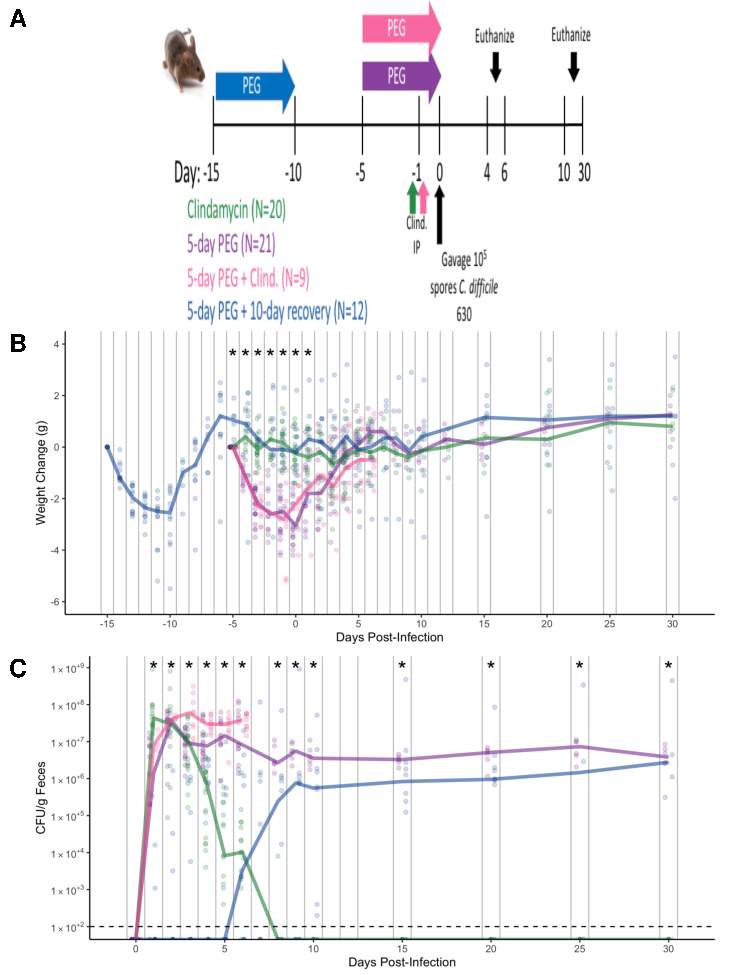
\includegraphics{figure_1.pdf}

\textbf{Figure 1. 5-day PEG treatment prolongs susceptibility and mice
become persistently colonized with \emph{C. difficile}.} A. Setup of the
experimental timeline for experiments with 5-day PEG treated mice.
Clindamycin was administered at 10 mg/kg by intraperitoneal injection.
15\% PEG 3350 was administered in the drinking water for five days. B.
Weight change from baseline weight in groups after treatment with PEG
and/or clindamycin, followed by \emph{C. difficile} challenge. C.
\emph{C. difficile} CFU/gram stool measured over time (N = 16-59 mice
per timepoint) via serial dilutions. The black line represents the limit
of detection for the first serial dilution. CFU quantification data was
not available for each mouse due to stool sampling difficulties
(particularly the day the mice came off of the PEG treatment) or early
deaths. For B-C, lines represent the median for each treatment group and
circles represent samples from individual mice. Asterisks indicate
timepoints where the weight change or CFU/g was significantly different
between groups by the Kruskal-Wallis test with Benjamini-Hochberg
correction for testing multiple timepoints. The data presented are from
a total of 5 separate experiments. \newpage

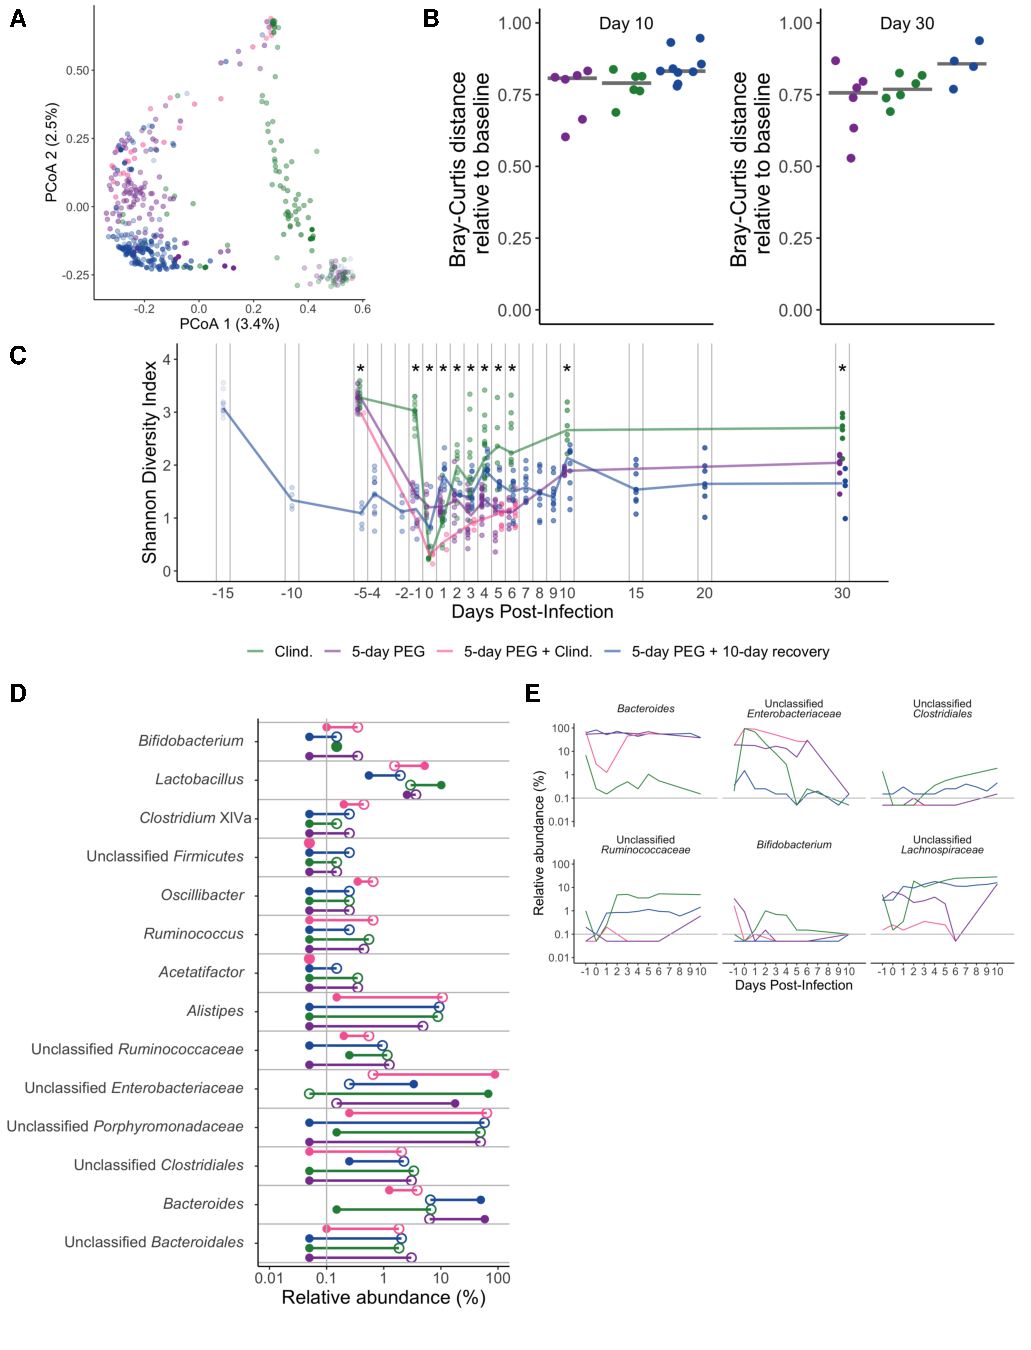
\includegraphics{figure_2.pdf} \textbf{Figure 2. 5-day PEG treatment
disrupts the stool microbiota for a longer amount of time compared to
clindamycin-treated mice.} A. PCoA of Bray-Curtis distances from stool
samples collected throughout the experiment. \newpage

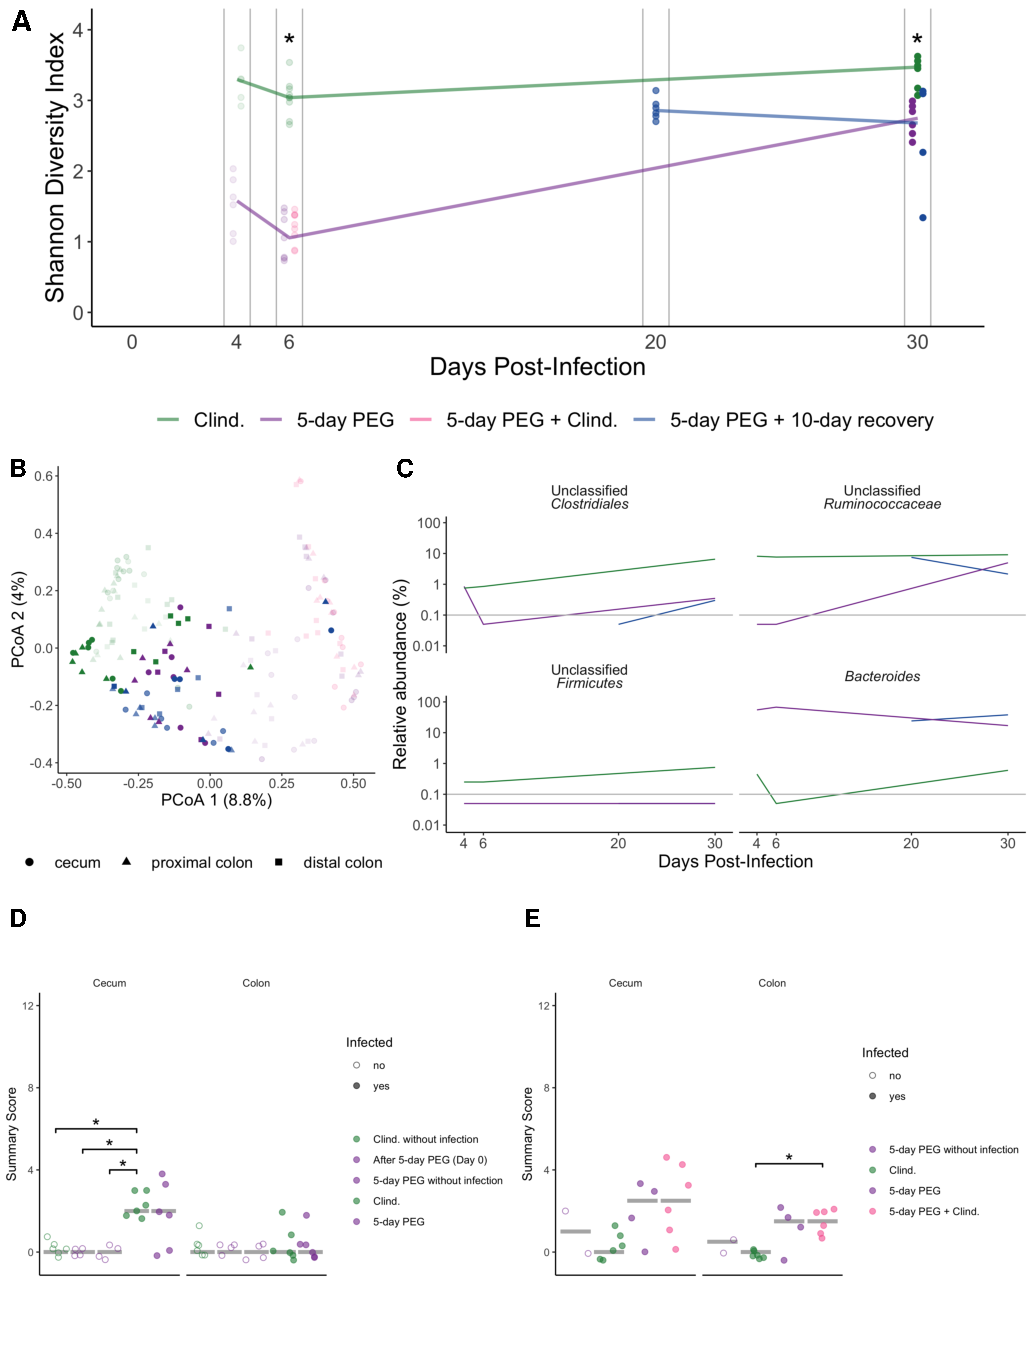
\includegraphics{figure_3.pdf} \textbf{Figure 3. 5-day PEG treatment
does not result in more severe CDIs, although mucosal microbiota is
altered.} A. \newpage

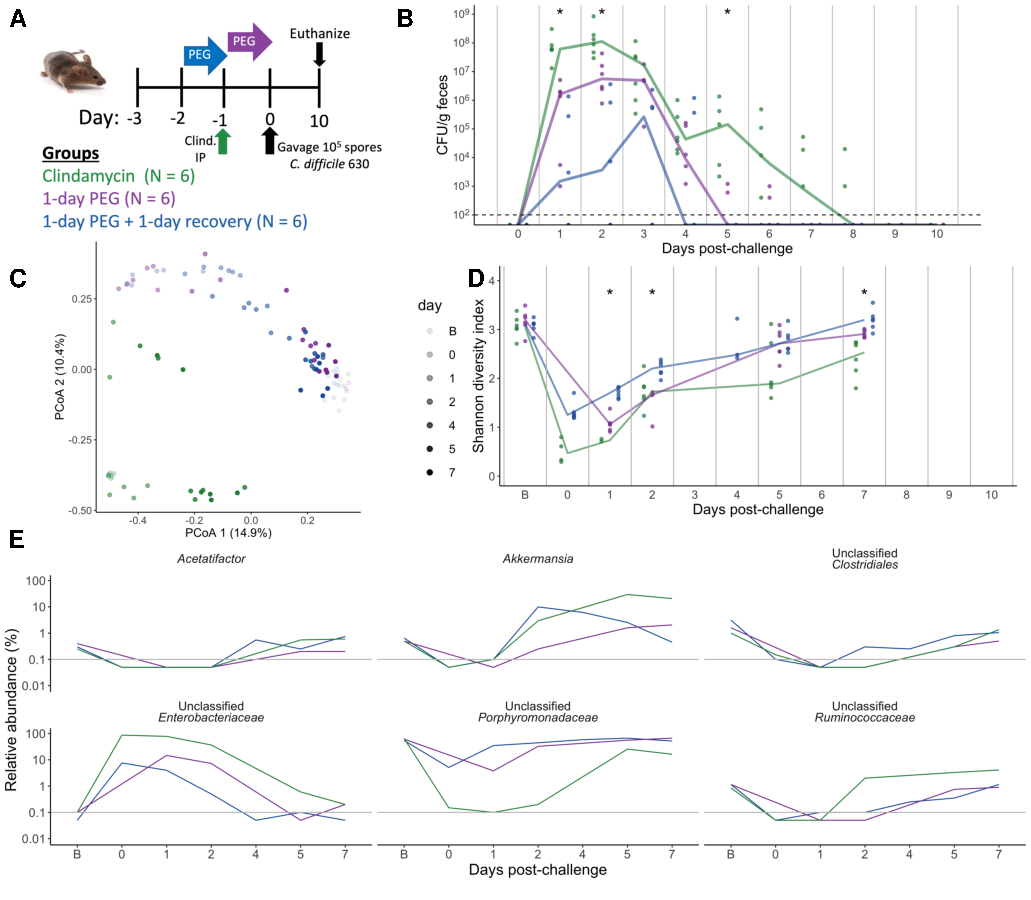
\includegraphics{figure_4.pdf} \textbf{Figure 4. 1-day PEG treatment
renders mice susceptible to transient \emph{C. difficile} colonization.}
A. Setup of the experimental timeline for the 1-day PEG treated subset
of mice. B. CFU/gram stool measured over time (N = 12-18 mice per
timepoint) via several dilutions. The black dotted line represents the
limit of detection for the first serial dilution. Asterisks indicate
timepoints where the CFU/gram was significantly different between groups
using the Kruskall-Wallis test with a Benjamini-Hochberg correction for
multiple timepoints. C. Principle Coordinate Analysis plot of the groups
over time with the alpha representating the same time scale as in panel
D (day: R\textsuperscript{2} = 0.43; group: R\textsuperscript{2} =
0.19). D. Shannon diversity Index of the groups over time. Only days
with samples from all groups are shown. E. Line plots of relative
percent abundance of selected genera over time. Only days with samples
from all groups shown. The gray line represents the limit of detection.

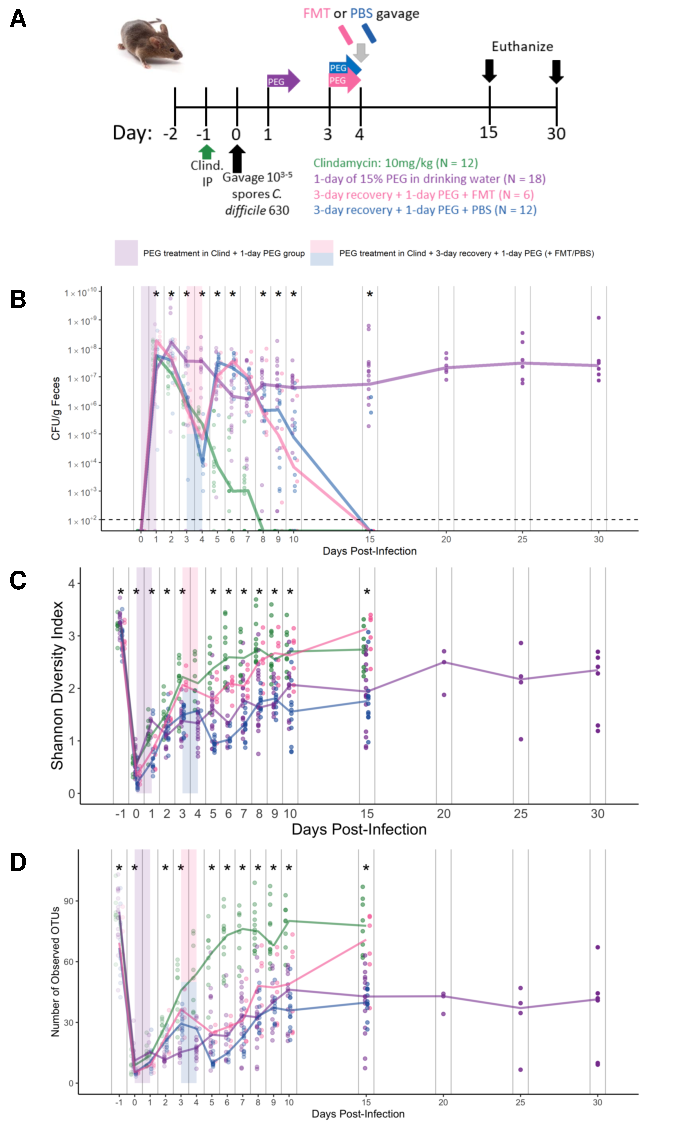
\includegraphics{figure_5.pdf} A. Experimental timeline for groups
receiving PEG treatment post clindamycin gavage. B. Median and
individual CFU/g of C. difficile measured over time via culture.
Asterisks indicate time points with significant differences between
groups using Kruskall-Wallis tests with a Benjamini-Hochberg correction.
Limit of detection is 1e2 CFU/g. Background shading indicates PEG
treatment period for applicable groups. Opacity of points reflects time
point. C. Median and individual Shannon Diversity measured over time.
Asterisks, background shading, and opacity of points consistent with
(B). D. Median and individual richness measured over time. Asterisks,
background shading, and opacity of points consistent with (B).

\newpage

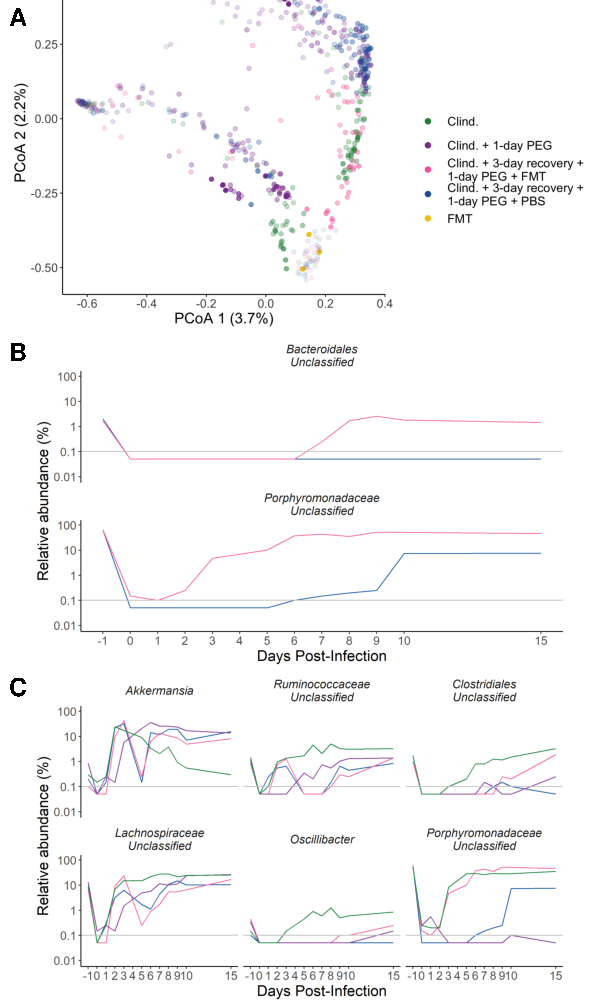
\includegraphics{figure_5_16S.pdf} \textbf{Figure 5. 1-day PEG treatment
post C. difficile challenge prolongs colonization regardless of whether
an FMT is also administered.} A. PCoA of all groups + FMT plotted over
time. Opacity of points reflects time point. B. Relative abundance of
genera significantly different over multiple time points post FMT or PBS
treatment, plotted over time. Limit of detection is .1\%. C. Relative
abundances of top 6 significant genera ranked by number of days
significant, plotted over time. Limit of detection is .1\%.

\newpage

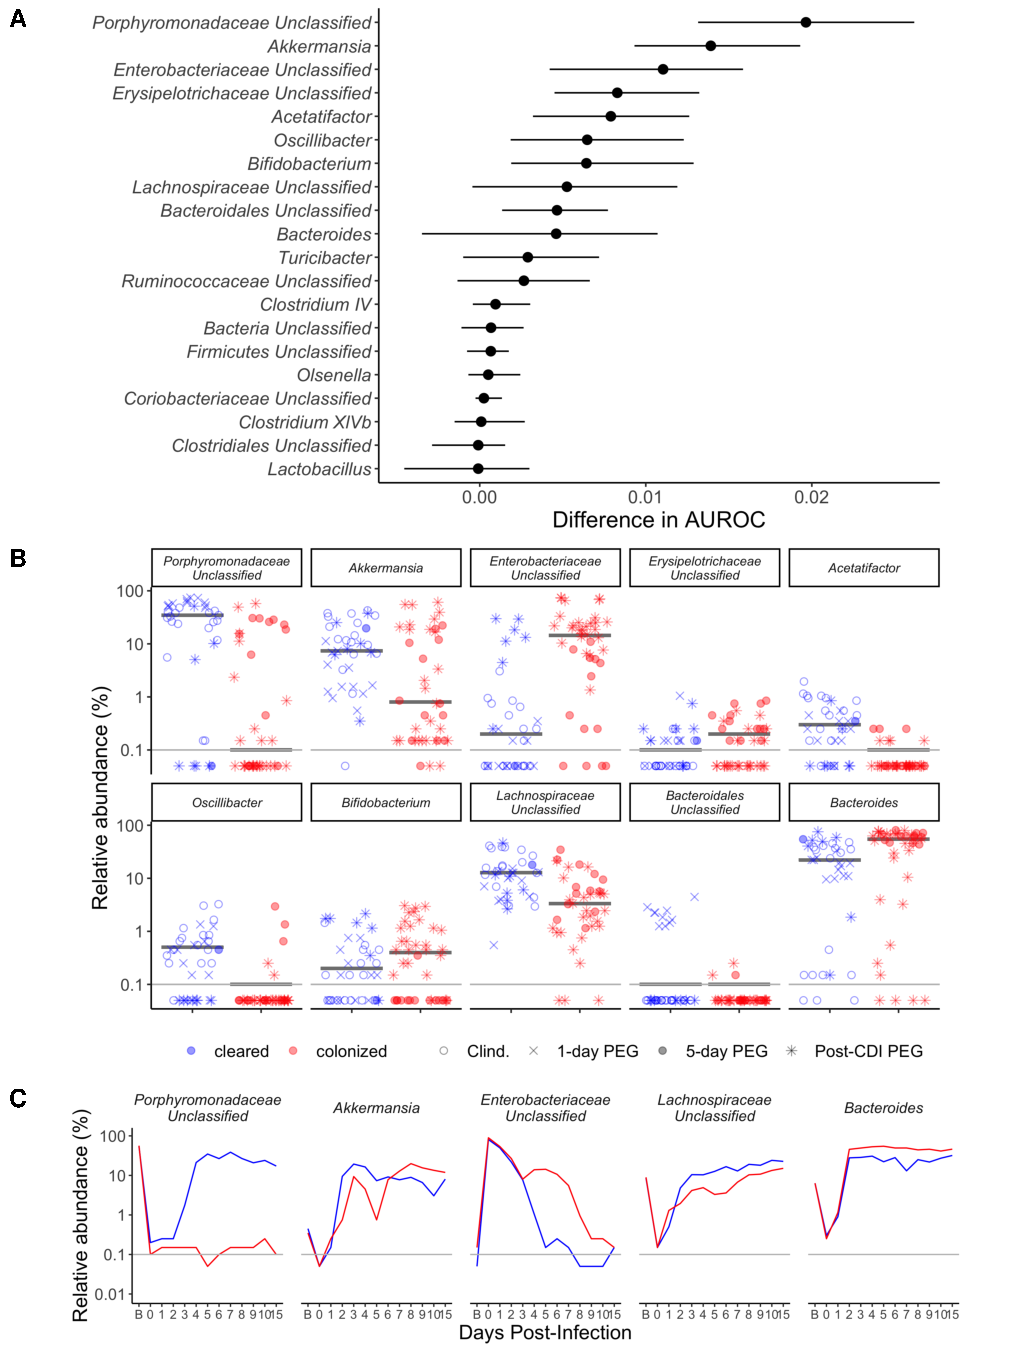
\includegraphics{figure_6.pdf} \textbf{Figure 6. Specific microbiota
features associated with prolonged \emph{C. difficile} colonization in
PEG treated mice.} A. \newpage

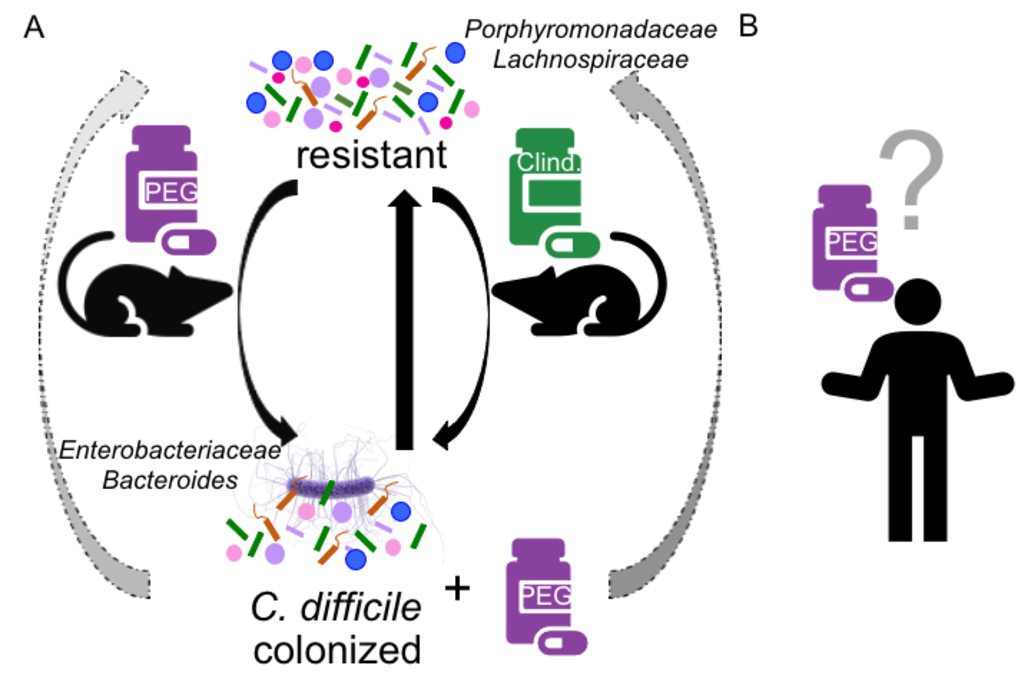
\includegraphics{figure_7.pdf} \textbf{Figure 7. Schematic summarizing
findings.} A. \newpage

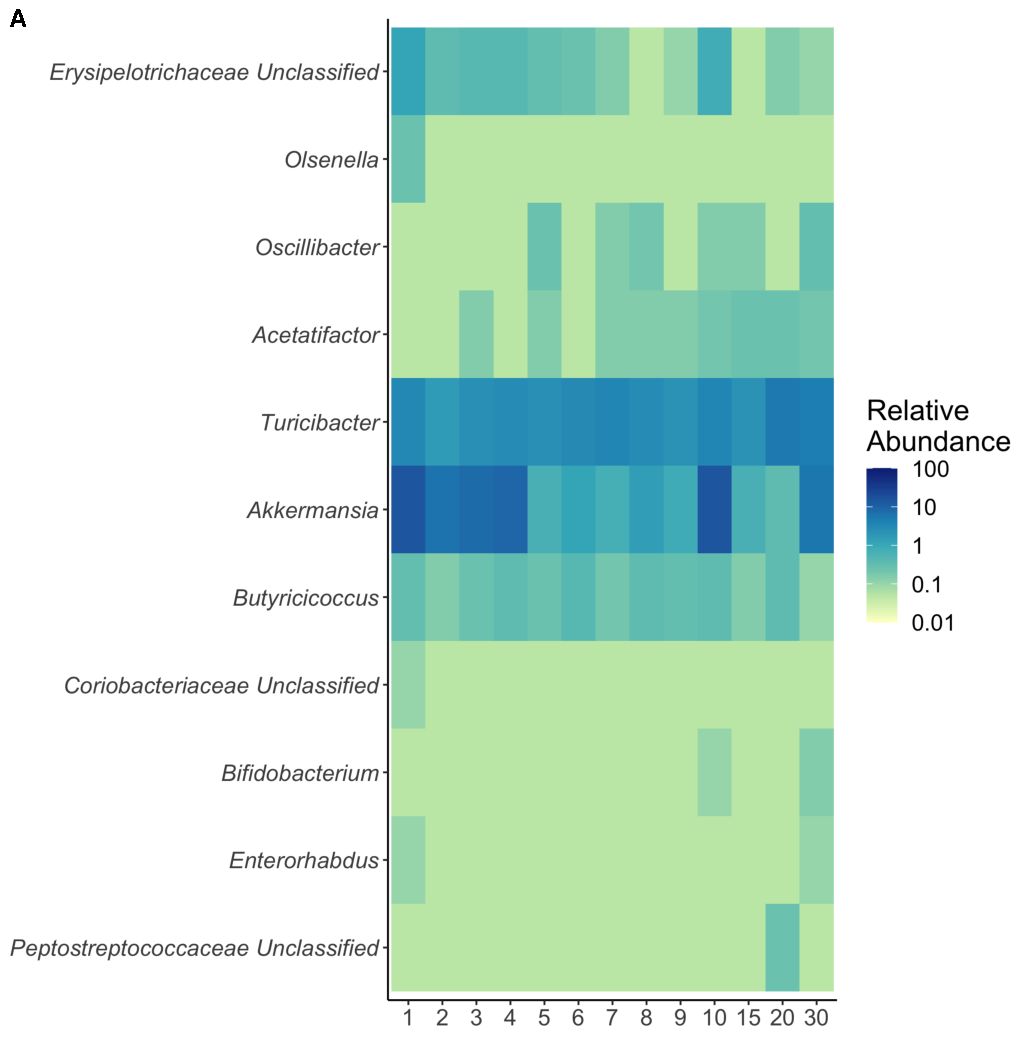
\includegraphics{figure_S1.pdf} \textbf{Figure S1. 5-day PEG treatment
plus 10-day recovery mice microbiota dynamics post-infection.} A.
\newpage

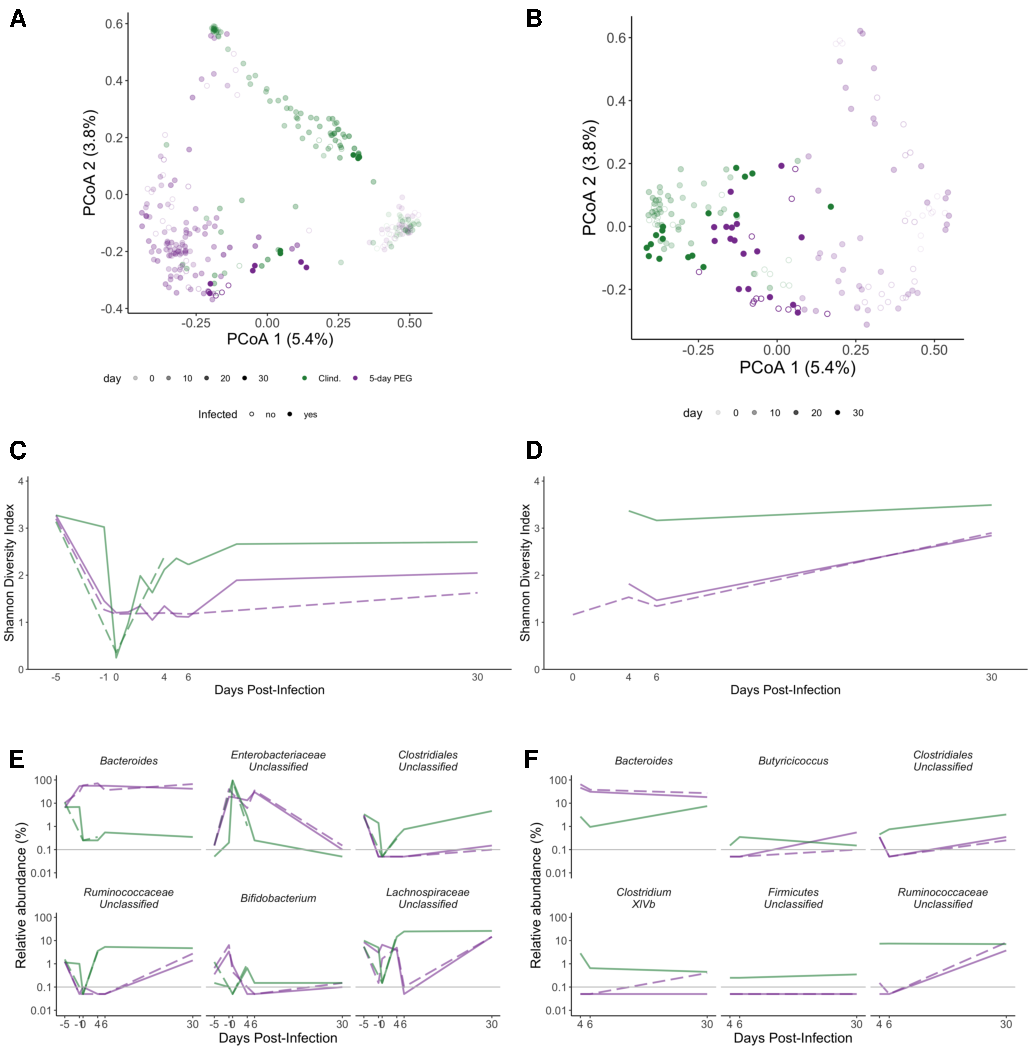
\includegraphics{figure_S2.pdf} \textbf{Figure S2. Specific OTUs
associated with clearance that are mostly absent in mice with prolonged
\emph{C. difficile} colonization. Ex. \emph{Muribaculum intestinale}.}
A. \newpage

\hypertarget{references}{%
\subsection*{References}\label{references}}
\addcontentsline{toc}{subsection}{References}

\hypertarget{refs}{}
\leavevmode\hypertarget{ref-Britton2014}{}%
1. \textbf{Britton RA}, \textbf{Young VB}. 2014. Role of the intestinal
microbiota in resistance to colonization by clostridium difficile.
Gastroenterology \textbf{146}:1547--1553.
doi:\href{https://doi.org/10.1053/j.gastro.2014.01.059}{10.1053/j.gastro.2014.01.059}.

\leavevmode\hypertarget{ref-Maier2018}{}%
2. \textbf{Maier L}, \textbf{Pruteanu M}, \textbf{Kuhn M},
\textbf{Zeller G}, \textbf{Telzerow A}, \textbf{Anderson EE},
\textbf{Brochado AR}, \textbf{Fernandez KC}, \textbf{Dose H},
\textbf{Mori H}, \textbf{Patil KR}, \textbf{Bork P}, \textbf{Typas A}.
2018. Extensive impact of non-antibiotic drugs on human gut bacteria.
Nature \textbf{555}:623--628.
doi:\href{https://doi.org/10.1038/nature25979}{10.1038/nature25979}.

\leavevmode\hypertarget{ref-LeBastard2017}{}%
3. \textbf{Bastard QL}, \textbf{Al-Ghalith GA}, \textbf{Grégoire M},
\textbf{Chapelet G}, \textbf{Javaudin F}, \textbf{Dailly E},
\textbf{Batard E}, \textbf{Knights D}, \textbf{Montassier E}. 2017.
Systematic review: Human gut dysbiosis induced by non-antibiotic
prescription medications. Alimentary Pharmacology \& Therapeutics
\textbf{47}:332--345.
doi:\href{https://doi.org/10.1111/apt.14451}{10.1111/apt.14451}.

\leavevmode\hypertarget{ref-VichVila2020}{}%
4. \textbf{Vila AV}, \textbf{Collij V}, \textbf{Sanna S}, \textbf{Sinha
T}, \textbf{Imhann F}, \textbf{Bourgonje AR}, \textbf{Mujagic Z},
\textbf{Jonkers DMAE}, \textbf{Masclee AAM}, \textbf{Fu J},
\textbf{Kurilshikov A}, \textbf{Wijmenga C}, \textbf{Zhernakova A},
\textbf{Weersma RK}. 2020. Impact of commonly used drugs on the
composition and metabolic function of the gut microbiota. Nature
Communications \textbf{11}.
doi:\href{https://doi.org/10.1038/s41467-019-14177-z}{10.1038/s41467-019-14177-z}.

\leavevmode\hypertarget{ref-Oh2018}{}%
5. \textbf{Oh J}, \textbf{Makar M}, \textbf{Fusco C}, \textbf{McCaffrey
R}, \textbf{Rao K}, \textbf{Ryan EE}, \textbf{Washer L}, \textbf{West
LR}, \textbf{Young VB}, \textbf{Guttag J}, \textbf{Hooper DC},
\textbf{Shenoy ES}, \textbf{Wiens J}. 2018. A generalizable, data-driven
approach to predict daily risk ofClostridium difficileInfection at two
large academic health centers. Infection Control \& Hospital
Epidemiology \textbf{39}:425--433.
doi:\href{https://doi.org/10.1017/ice.2018.16}{10.1017/ice.2018.16}.

\leavevmode\hypertarget{ref-Mora2012}{}%
6. \textbf{Mora AL}, \textbf{Salazar M}, \textbf{Pablo-Caeiro J},
\textbf{Frost CP}, \textbf{Yadav Y}, \textbf{DuPont HL}, \textbf{Garey
KW}. 2012. Moderate to high use of opioid analgesics are associated with
an increased risk of clostridium difficile infection. The American
Journal of the Medical Sciences \textbf{343}:277--280.
doi:\href{https://doi.org/10.1097/maj.0b013e31822f42eb}{10.1097/maj.0b013e31822f42eb}.

\leavevmode\hypertarget{ref-Nehra2018}{}%
7. \textbf{Nehra AK}, \textbf{Alexander JA}, \textbf{Loftus CG},
\textbf{Nehra V}. 2018. Proton pump inhibitors: Review of emerging
concerns. Mayo Clinic Proceedings \textbf{93}:240--246.
doi:\href{https://doi.org/10.1016/j.mayocp.2017.10.022}{10.1016/j.mayocp.2017.10.022}.

\leavevmode\hypertarget{ref-Krishna2013}{}%
8. \textbf{Krishna SG}, \textbf{Zhao W}, \textbf{Apewokin SK},
\textbf{Krishna K}, \textbf{Chepyala P}, \textbf{Anaissie EJ}. 2013.
Risk factors, preemptive therapy, and antiperistaltic agents
forClostridium difficileinfection in cancer patients. Transplant
Infectious Disease n/a--n/a.
doi:\href{https://doi.org/10.1111/tid.12112}{10.1111/tid.12112}.

\leavevmode\hypertarget{ref-Tomkovich2019}{}%
9. \textbf{Tomkovich S}, \textbf{Lesniak NA}, \textbf{Li Y},
\textbf{Bishop L}, \textbf{Fitzgerald MJ}, \textbf{Schloss PD}. 2019.
The proton pump inhibitor omeprazole does not promote
\emph{Clostridioides difficile} colonization in a murine model. mSphere
\textbf{4}.
doi:\href{https://doi.org/10.1128/msphere.00693-19}{10.1128/msphere.00693-19}.

\leavevmode\hypertarget{ref-Vandeputte2015}{}%
10. \textbf{Vandeputte D}, \textbf{Falony G}, \textbf{Vieira-Silva S},
\textbf{Tito RY}, \textbf{Joossens M}, \textbf{Raes J}. 2015. Stool
consistency is strongly associated with gut microbiota richness and
composition, enterotypes and bacterial growth rates. Gut
\textbf{65}:57--62.
doi:\href{https://doi.org/10.1136/gutjnl-2015-309618}{10.1136/gutjnl-2015-309618}.

\leavevmode\hypertarget{ref-VujkovicCvijin2020}{}%
11. \textbf{Vujkovic-Cvijin I}, \textbf{Sklar J}, \textbf{Jiang L},
\textbf{Natarajan L}, \textbf{Knight R}, \textbf{Belkaid Y}. 2020. Host
variables confound gut microbiota studies of human disease. Nature
\textbf{587}:448--454.
doi:\href{https://doi.org/10.1038/s41586-020-2881-9}{10.1038/s41586-020-2881-9}.

\leavevmode\hypertarget{ref-Schubert2015}{}%
12. \textbf{Schubert AM}, \textbf{Sinani H}, \textbf{Schloss PD}. 2015.
Antibiotic-induced alterations of the murine gut microbiota and
subsequent effects on colonization resistance against \emph{Clostridium
difficile}. mBio \textbf{6}.
doi:\href{https://doi.org/10.1128/mbio.00974-15}{10.1128/mbio.00974-15}.

\leavevmode\hypertarget{ref-Nagata2019}{}%
13. \textbf{Nagata N}, \textbf{Tohya M}, \textbf{Fukuda S}, \textbf{Suda
W}, \textbf{Nishijima S}, \textbf{Takeuchi F}, \textbf{Ohsugi M},
\textbf{Tsujimoto T}, \textbf{Nakamura T}, \textbf{Shimomura A},
\textbf{Yanagisawa N}, \textbf{Hisada Y}, \textbf{Watanabe K},
\textbf{Imbe K}, \textbf{Akiyama J}, \textbf{Mizokami M},
\textbf{Miyoshi-Akiyama T}, \textbf{Uemura N}, \textbf{Hattori M}. 2019.
Effects of bowel preparation on the human gut microbiome and metabolome.
Scientific Reports \textbf{9}.
doi:\href{https://doi.org/10.1038/s41598-019-40182-9}{10.1038/s41598-019-40182-9}.

\leavevmode\hypertarget{ref-Kashyap2013}{}%
14. \textbf{Kashyap PC}, \textbf{Marcobal A}, \textbf{Ursell LK},
\textbf{Larauche M}, \textbf{Duboc H}, \textbf{Earle KA},
\textbf{Sonnenburg ED}, \textbf{Ferreyra JA}, \textbf{Higginbottom SK},
\textbf{Million M}, \textbf{Tache Y}, \textbf{Pasricha PJ},
\textbf{Knight R}, \textbf{Farrugia G}, \textbf{Sonnenburg JL}. 2013.
Complex interactions among diet, gastrointestinal transit, and gut
microbiota in humanized mice. Gastroenterology \textbf{144}:967--977.
doi:\href{https://doi.org/10.1053/j.gastro.2013.01.047}{10.1053/j.gastro.2013.01.047}.

\leavevmode\hypertarget{ref-Ferreyra2014}{}%
15. \textbf{Ferreyra JA}, \textbf{Wu KJ}, \textbf{Hryckowian AJ},
\textbf{Bouley DM}, \textbf{Weimer BC}, \textbf{Sonnenburg JL}. 2014.
Gut microbiota-produced succinate promotes c.~difficile infection after
antibiotic treatment or motility disturbance. Cell Host \& Microbe
\textbf{16}:770--777.
doi:\href{https://doi.org/10.1016/j.chom.2014.11.003}{10.1016/j.chom.2014.11.003}.

\leavevmode\hypertarget{ref-Tropini2018}{}%
16. \textbf{Tropini C}, \textbf{Moss EL}, \textbf{Merrill BD},
\textbf{Ng KM}, \textbf{Higginbottom SK}, \textbf{Casavant EP},
\textbf{Gonzalez CG}, \textbf{Fremin B}, \textbf{Bouley DM},
\textbf{Elias JE}, \textbf{Bhatt AS}, \textbf{Huang KC},
\textbf{Sonnenburg JL}. 2018. Transient osmotic perturbation causes
long-term alteration to the gut microbiota. Cell
\textbf{173}:1742--1754.e17.
doi:\href{https://doi.org/10.1016/j.cell.2018.05.008}{10.1016/j.cell.2018.05.008}.

\leavevmode\hypertarget{ref-VanInsberghe2020}{}%
17. \textbf{VanInsberghe D}, \textbf{Elsherbini JA}, \textbf{Varian B},
\textbf{Poutahidis T}, \textbf{Erdman S}, \textbf{Polz MF}. 2020.
Diarrhoeal events can trigger long-term clostridium difficile
colonization with recurrent blooms. Nature Microbiology
\textbf{5}:642--650.
doi:\href{https://doi.org/10.1038/s41564-020-0668-2}{10.1038/s41564-020-0668-2}.

\leavevmode\hypertarget{ref-Liacouras1996}{}%
18. \textbf{Liacouras CA}, \textbf{Piccoli DA}. 1996. Whole-bowel
irrigation as an adjunct to the treatment of chronic, relapsing
clostridium difficile colitis. Journal of Clinical Gastroenterology
\textbf{22}:186--189.
doi:\href{https://doi.org/10.1097/00004836-199604000-00007}{10.1097/00004836-199604000-00007}.

\leavevmode\hypertarget{ref-Tomkovich2020}{}%
19. \textbf{Tomkovich S}, \textbf{Stough JMA}, \textbf{Bishop L},
\textbf{Schloss PD}. 2020. The initial gut microbiota and response to
antibiotic perturbation influence clostridioides difficile clearance in
mice. mSphere \textbf{5}.
doi:\href{https://doi.org/10.1128/msphere.00869-20}{10.1128/msphere.00869-20}.

\leavevmode\hypertarget{ref-Reeves2011}{}%
20. \textbf{Reeves AE}, \textbf{Theriot CM}, \textbf{Bergin IL},
\textbf{Huffnagle GB}, \textbf{Schloss PD}, \textbf{Young VB}. 2011. The
interplay between microbiome dynamics and pathogen dynamics in a murine
model of \emph{Clostridium difficile} infection \textbf{2}:145--158.
doi:\href{https://doi.org/10.4161/gmic.2.3.16333}{10.4161/gmic.2.3.16333}.

\leavevmode\hypertarget{ref-Jenior2018}{}%
21. \textbf{Jenior ML}, \textbf{Leslie JL}, \textbf{Young VB},
\textbf{Schloss PD}. 2018. \emph{Clostridium difficile} alters the
structure and metabolism of distinct cecal microbiomes during initial
infection to promote sustained colonization. mSphere \textbf{3}.
doi:\href{https://doi.org/10.1128/msphere.00261-18}{10.1128/msphere.00261-18}.

\leavevmode\hypertarget{ref-Vornhagen2020}{}%
22. \textbf{Vornhagen J}, \textbf{Bassis CM}, \textbf{Ramakrishnan S},
\textbf{Hein R}, \textbf{Mason S}, \textbf{Bergman Y}, \textbf{Sunshine
N}, \textbf{Fan Y}, \textbf{Timp W}, \textbf{Schatz MC}, \textbf{Young
VB}, \textbf{Simner PJ}, \textbf{Bachman MA}. 2020. A plasmid locus
associated with klebsiella clinical infections encodes a
microbiome-dependent gut fitness factor.
doi:\href{https://doi.org/10.1101/2020.02.26.963322}{10.1101/2020.02.26.963322}.

\end{document}
